% comment out (using a %) exactly 1 of the 2 lines immediately below
%\documentclass[handout]{beamer}   % to produce a handout
\documentclass{beamer}             % to produce slide show with pauses etc.

%\usepackage{xeCJK}
%\setCJKmainfont{SimSun}

\usepackage{ucltemplate}
\usepackage{hyperref}  % to enable hyperlinks to websites to be produced.
   \usepackage[utf8]{inputenc}

\setbeamertemplate{footline}{\normalsize\hfill\insertframenumber/\inserttotalframenumber} % add slide number

\newenvironment{conditions}[1][where:]
{%
	#1\tabularx{\textwidth-\widthof{#1}}[t]{
		>{$}l<{$} @{${}={}$} X@{}
	}%
}
{\endtabularx\\[\belowdisplayskip]}

\setbeamertemplate{navigation symbols}{} %no navigation symbols on the bottom right of the slides

% To force beamer to include table and figure numbers
% This is just for the purposes of the STAT0034 workshop: usually one would not want cross-references in a presentation
\setbeamertemplate{caption}[numbered]

% for nice-looking inequality signs
\let\leq=\leqslant
\let\geq=\geqslant

% Choose the color you like
\usecolortheme{lightblue}
%\usecolortheme{black}
%\usecolortheme{darkred}

% Pick a colour (a blue) for the weblinks
\definecolor{links}{HTML}{2B65EC}
\hypersetup{colorlinks, linkcolor=, urlcolor = links}

% Information for title page
\title{\bf The NIR Corn Data Set}
\author{Hongwei PENG \vspace{1cm} \\
	Supervisor : Prof Tom Fearn\\
	Department of Statistical Science \\
	University College London}
\institute{Department of Statistical Science}
\date{\today}

% Start the document
\begin{document}
	
	
\begin{frame}
	\titlepage
\end{frame}	
	
	\begin{frame}{Datasets}
	Corn data is the most readily available high-dimensional Near-infrared spectral data. This data was published on the Internet (http://www.eigenvector.com/data/Corn/index.html) by Eigenvector Research, Inc. in 2005. The data consisted of 80 corn samples measured on three different NIR spectrometers named m5, mp5 and mp6. The spectral wavelength range is 1100$\sim$2498nm with an interval of 2nm. Hence there are 700 channels for each spectrum in each sample. Figure is the plot of spectra on m5 and mp5.
\end{frame}

	
\begin{frame}{Datasets}
	
	% A picture can be included as an pdf using \includegraphics
	% The construction below with tabular and minipage is one
	% way to create a good layout.
	\begin{tabular}{cc}
		\begin{minipage}{2in}
			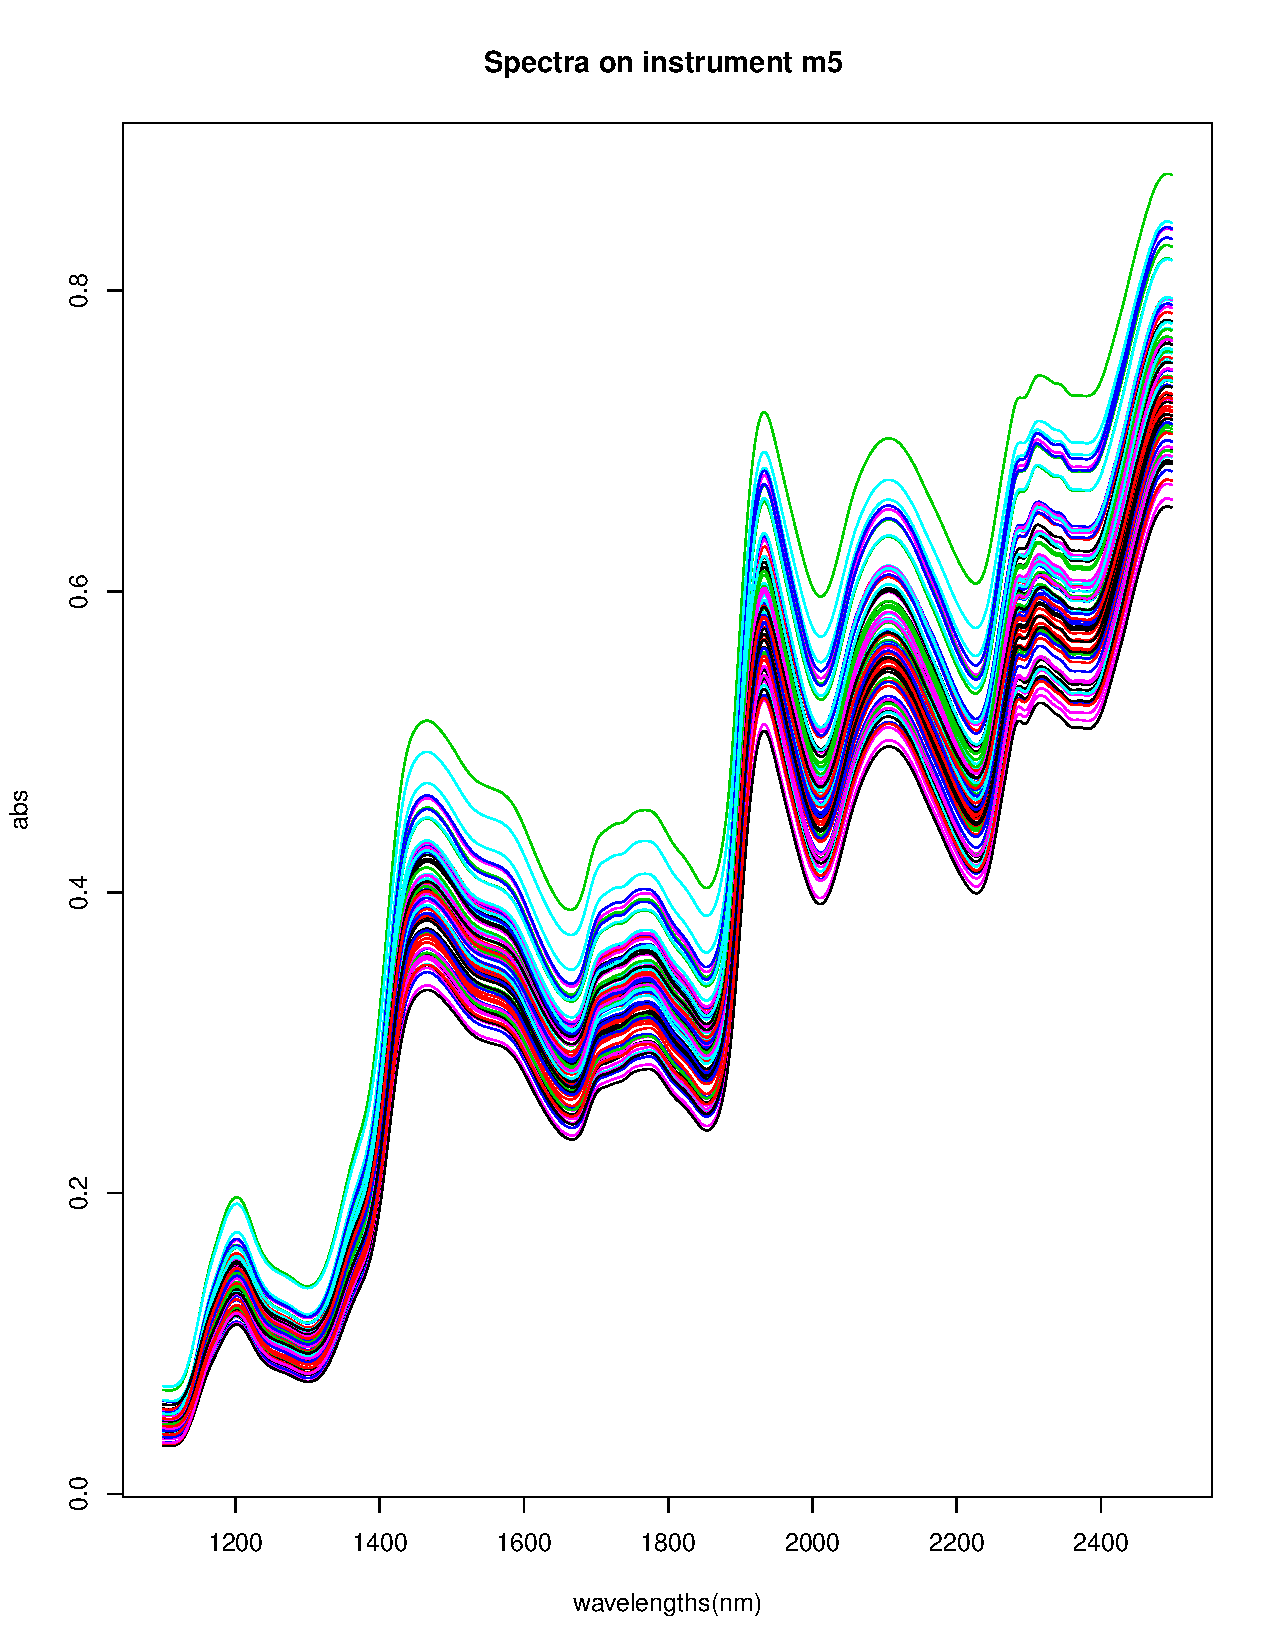
\includegraphics[width=2.2in]{Spectra_on_instrument_m5.pdf}
		\end{minipage}
		&
		\begin{minipage}{2in}
			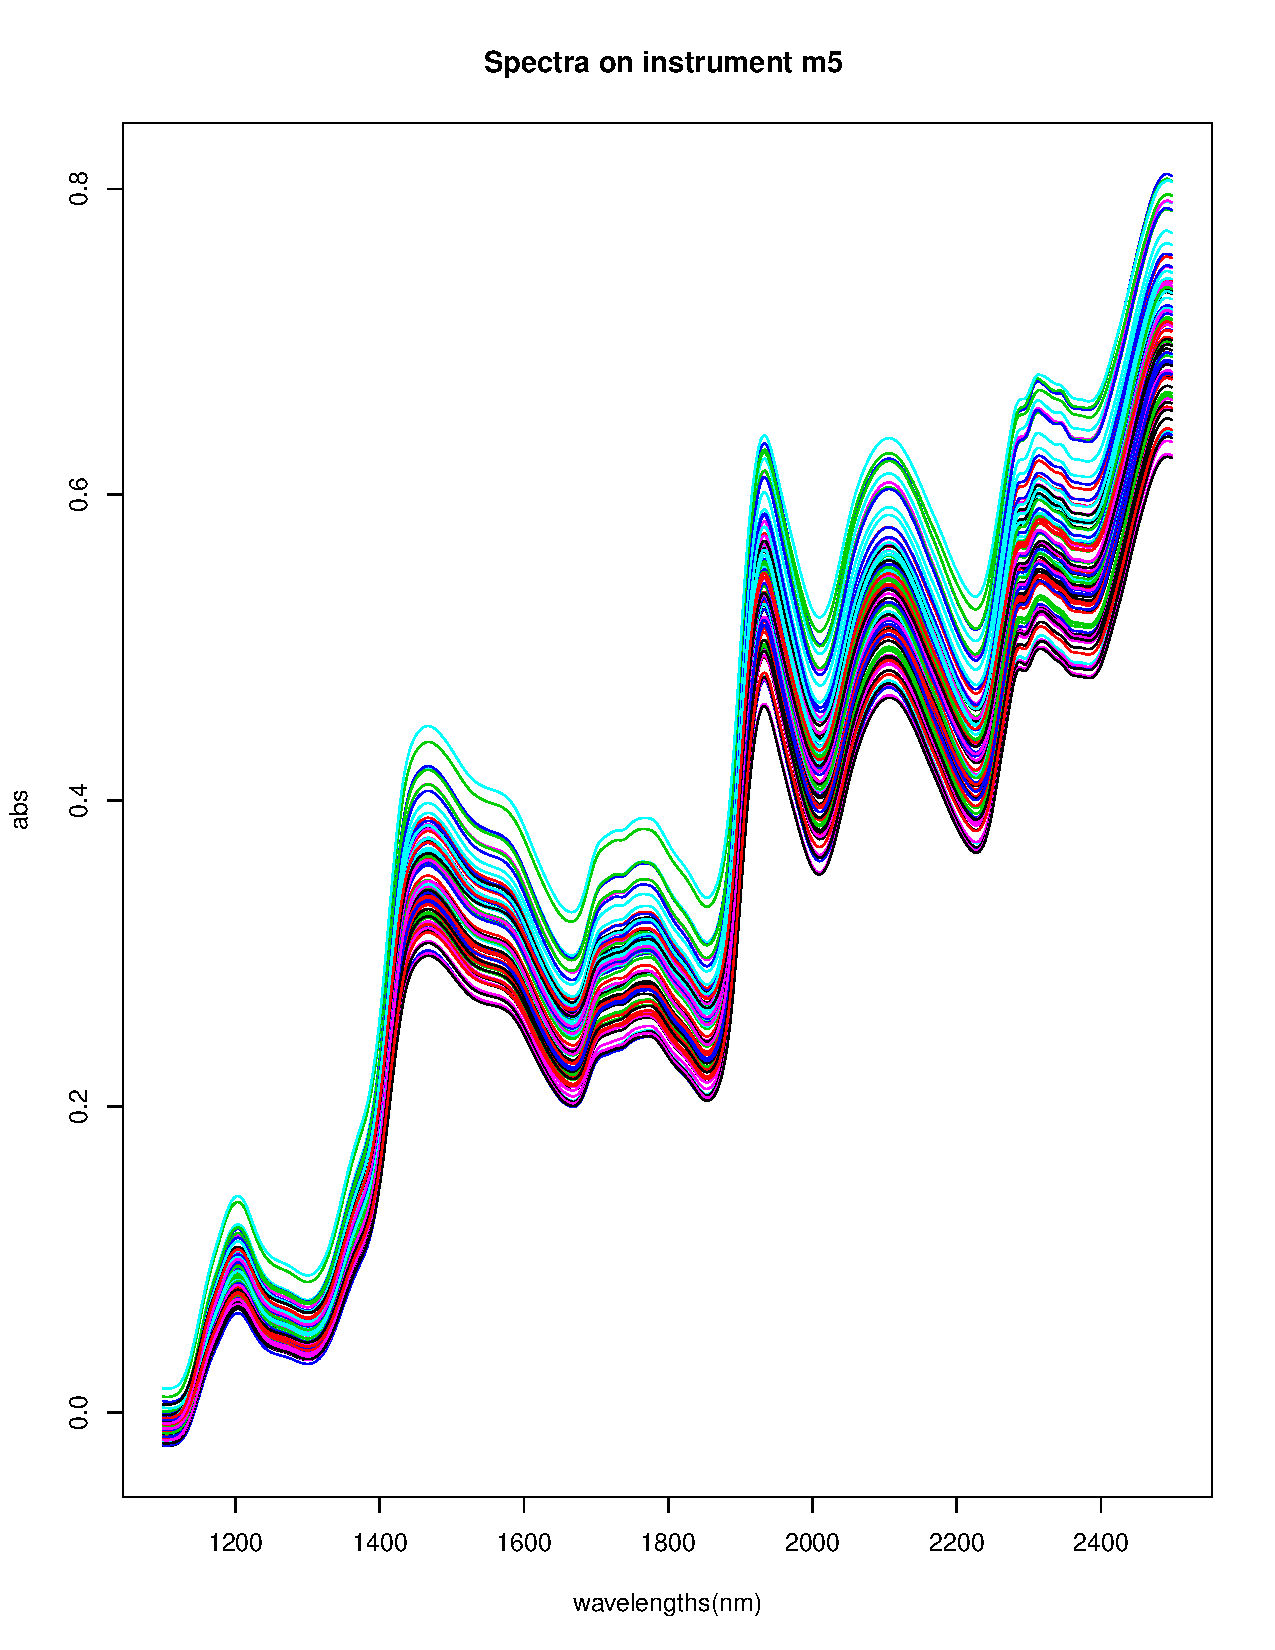
\includegraphics[width=2.2in]{Spectra_on_instrument_mp5.pdf}
		\end{minipage}
	\end{tabular}
\end{frame}


		\begin{frame}
				\begin{tabular}{cc}
					\begin{minipage}{5in}
				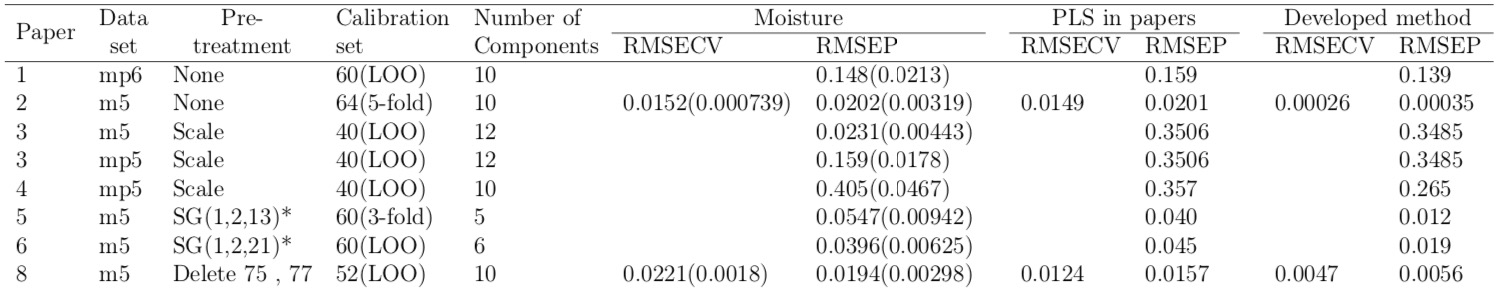
\includegraphics[width=4.3in]{tab-moisture.png}
					\end{minipage}
					\end{tabular}
		\end{frame}




	\begin{frame}[containsverbatim]{Compare with papers}
		
\begin{table}[h]
	\centering           % put the graph(s) in the centre of the page (horizontally)
	
	\begin{tabular}{llllll}
		
		\hline
		\multicolumn{1}{c}{Paper} & \begin{tabular}[c]{@{}l@{}}Prediction\\ set\end{tabular} & \begin{tabular}[c]{@{}l@{}}RMSEP\\ of PLS in\\ papers\end{tabular} & \begin{tabular}[c]{@{}l@{}}RMSEP of\\ developed\\ method\end{tabular} & F value & \begin{tabular}[c]{@{}l@{}}Significant \\ F statistic\\ (0.05)\end{tabular} \\ \hline
		1 & 20 & 0.159 & 0.139 & 1.31 & 2.124155 \\
		2 & 16 & 0.0201 & 0.00035 & 3298.04 & 2.333484 \\
		3 & 40 & 0.3506 & 0.3485 & 1.01 & 1.692797 \\
		4 & 40 & 0.357 & 0.265 & 1.81 & 1.692797 \\
		5 & 20 & 0.040 & 0.012 & 11.11 & 2.124155 \\
		6 & 20 & 0.045 & 0.019 & 5.61 & 2.124155 \\
		8 & 26 & 0.0157 & 0.0056 & 7.86 & 1.929213
	\end{tabular}
	\caption{F-test on regression of moisture.}
	\label{tab:F-moisture}
	
\end{table}
	
	\end{frame}
	
	\begin{frame}[containsverbatim]{Compare with papers}
	
		
	In section, although we calculated the difference between PLS and the developed method, there is no evaluation index to evaluate whether there is a significant difference between the two method. Because RMSEP does not obey the common distribution, which is why it is difficult to test, this section gives an approximate test method. This method is true when the model's bias is much smaller than the variance. According to section, RMSEP is calculated as follows, it can be divided into two parts, variance and bias.
	
	
	\begin{equation}
	RMSEP^2={\frac{1}{m}\sum_{i=1}^{m} (\hat y_i-y_i)^2}=Var(\hat{y})+Bias(\hat{y},y)^2 \approx Var(\hat{y})
	\end{equation}
	
	Here, if the model's bias is much smaller than the variance, then the BIOS can be ignored. Thus, RMSEP obeys the $\chi^2$ distribution. 
	
	\begin{equation}
	\dfrac{df*Var(\hat{y})}{\sigma} \sim \chi_{df}^2
	\end{equation}

	
	
	Therefore, the F-value corresponding to the chi-square distribution can be constructed to check whether the difference between the two groups is significant. F value structure is as follows.
	
	\begin{equation}
	\frac{RMSEP_{1}^{2}}{RMSEP_{2}^{2}} \sim F(df_1,df_2)
	\end{equation}

	
		\end{frame}


\end{document}



